\documentclass[12pt]{article}
\usepackage{amsmath}
\newcommand{\myvec}[1]{\ensuremath{\begin{pmatrix}#1\end{pmatrix}}}
\newcommand{\mydet}[1]{\ensuremath{\begin{vmatrix}#1\end{vmatrix}}}
\newcommand{\solution}{\noindent \textbf{Solution: }}
\providecommand{\brak}[1]{\ensuremath{\left(#1\right)}}
\providecommand{\norm}[1]{\left\lVert#1\right\rVert}
\let\vec\mathbf
\usepackage{graphicx}
\graphicspath{ {./images/} }

\title{Linear equation in two variables}
\author{potnuru deekshitha (potnurudeekshitha@sriprakashschools.com)}

\begin{document}
\maketitle
\section*{10$^{th}$ Maths - Chapter 7}
This is Problem-2 from Exercise 7.2
\begin{enumerate}
\item Find the coordinates of the point of trisection joining (4,-1),(-2,-3)
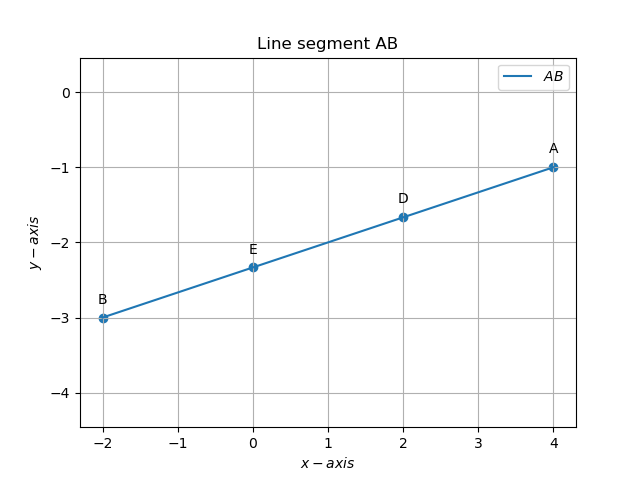
\includegraphics{/home/clab16/Documents/deekshitha py.png}
\solution\\
Case-1\\
$\vec{A}$=\myvec{4\\-2}, $\vec{B}$=\myvec{1\\-3},
$m_1:m_2=2:1$
\begin{align}
&P=\frac{m_1B+m_2A}{m_1+m_2}\\
&P=\frac{2\myvec{4\\-2}+1\myvec{-2\\-3}}{2+1}\\
&P=\frac{\myvec{8-2\\-4-3}}{2+1}\\
&P=\myvec{\frac{8-2}{2+1}\\\frac{-4-3}{2+1}}\\
&P=\myvec{\frac{6}{3}\\\frac{-7}{3}}\\
&P=\myvec{2\\\frac{-7}{3}}\\
\end{align}
Case-2\\
$\vec{A}$=\myvec{4\\-2}, $\vec{B}$=\myvec{1\\-3},
$m_1:m_2=1:2$
\begin{align}
&P=\frac{m_1B+m_2A}{m_1+m_2}\\
&P=\frac{1\myvec{4\\-2}+2\myvec{-2\\-3}}{1+2}\\
&P=\frac{\myvec{4-4\\-2-6}}{1+2}\\
&P=\myvec{\frac{4-4}{1+2}\\\frac{-2-6}{1+2}}\\
&P=\myvec{\frac{0}{3}\\\frac{-8}{3}}\\
&P=\myvec{0\\\frac{-8}{3}}\\
\end{align}
\end{enumerate}
\end{document}